\section{Auswertung der Messdaten}
\label{sec:Auswertung}

\subsection{Eichung des Magnetfeldes}
\label{sec:magnetfeld}
Die bei der Messung des Magnetfeldes aufgenommenen Daten sind in Tabelle \ref{tab:B} aufgelistet.

\begin{table}[H]
    \centering
      \caption{Magnetfeldstärke $B$ für verschiedene Stromstärken $I$.}
      \label{tab:B}
      \sisetup{table-format=3.1}
      \begin{tabular}{S[table-format=1.1] S}
        \toprule
        {$I[\si{\ampere}]$} & {$B[\si{\milli\tesla}]$}\\
        \midrule
        0   &   7.3    \\       
        1   &   106.2  \\
        2   &   206.2  \\
        3   &   301.9  \\
        4   &   388.4  \\
        5   &   462.8  \\
        6   &   522.9  \\
        7   &   560.2  \\
        7.5 &   577.5  \\
        \bottomrule
      \end{tabular}
\end{table}
\noindent

Für diese Messwerte wurde mittels \textit{numpy.polyfit} \cite{numpy} eine Regression der Form 
\begin{equation}
  B=aI^3+bI^2+cI+d \label{eqn:B}
\end{equation}
durchgeführt. Diese ist in Abbildung \ref{fig:B} visualisiert. 

\begin{figure}[H]
    \centering
    \includegraphics[scale= 0.8]{build/magnet.pdf}
    \caption{Magnetfeldstärke $B$ für verschiedene Stromstärken $I$ mit Regression.}
    \label{fig:B}
\end{figure}
\noindent

Die berechneten Parameter der Regression \ref{eqn:B} ergeben sich zu
\begin{align*}
    a&=\SI{-0.59\pm 0.06}{\milli\tesla\per\cubic\ampere}\\
    b&=\SI{1.20 \pm 0.66}{\milli\tesla\per\square\ampere}\\
    c&=\SI{99.91\pm 2.05}{\milli\tesla\per\ampere}\\
    d&=\SI{6.68 \pm 1.64}{\milli\tesla} .
\end{align*}

\subsection{Auswertung der roten Spektrallinie}
\label{sec:rot}
Für die rote Spektrallinie wurden während der Messung die Bilder \ref{fig:rot} und \ref{fig:rot_sigma} 
aufgenommenen. Dabei ist in Abbildung \ref{fig:rot} das Interferenzmuster ohne Magnetfeld und in 
Abbildung \ref{fig:rot_sigma} das Interferenzmuster mit Magnetfeld abegebildet. Der Elektromagnet wurde 
bei einer Stromstärke von $I=\SI{7.5}{\ampere}$ betrieben, was nach Kapitel \ref{sec:magnetfeld} einem 
Feld von $B=\SI{577.5}{\milli\tesla}$ entspricht.

\begin{figure}[H]
    \centering
    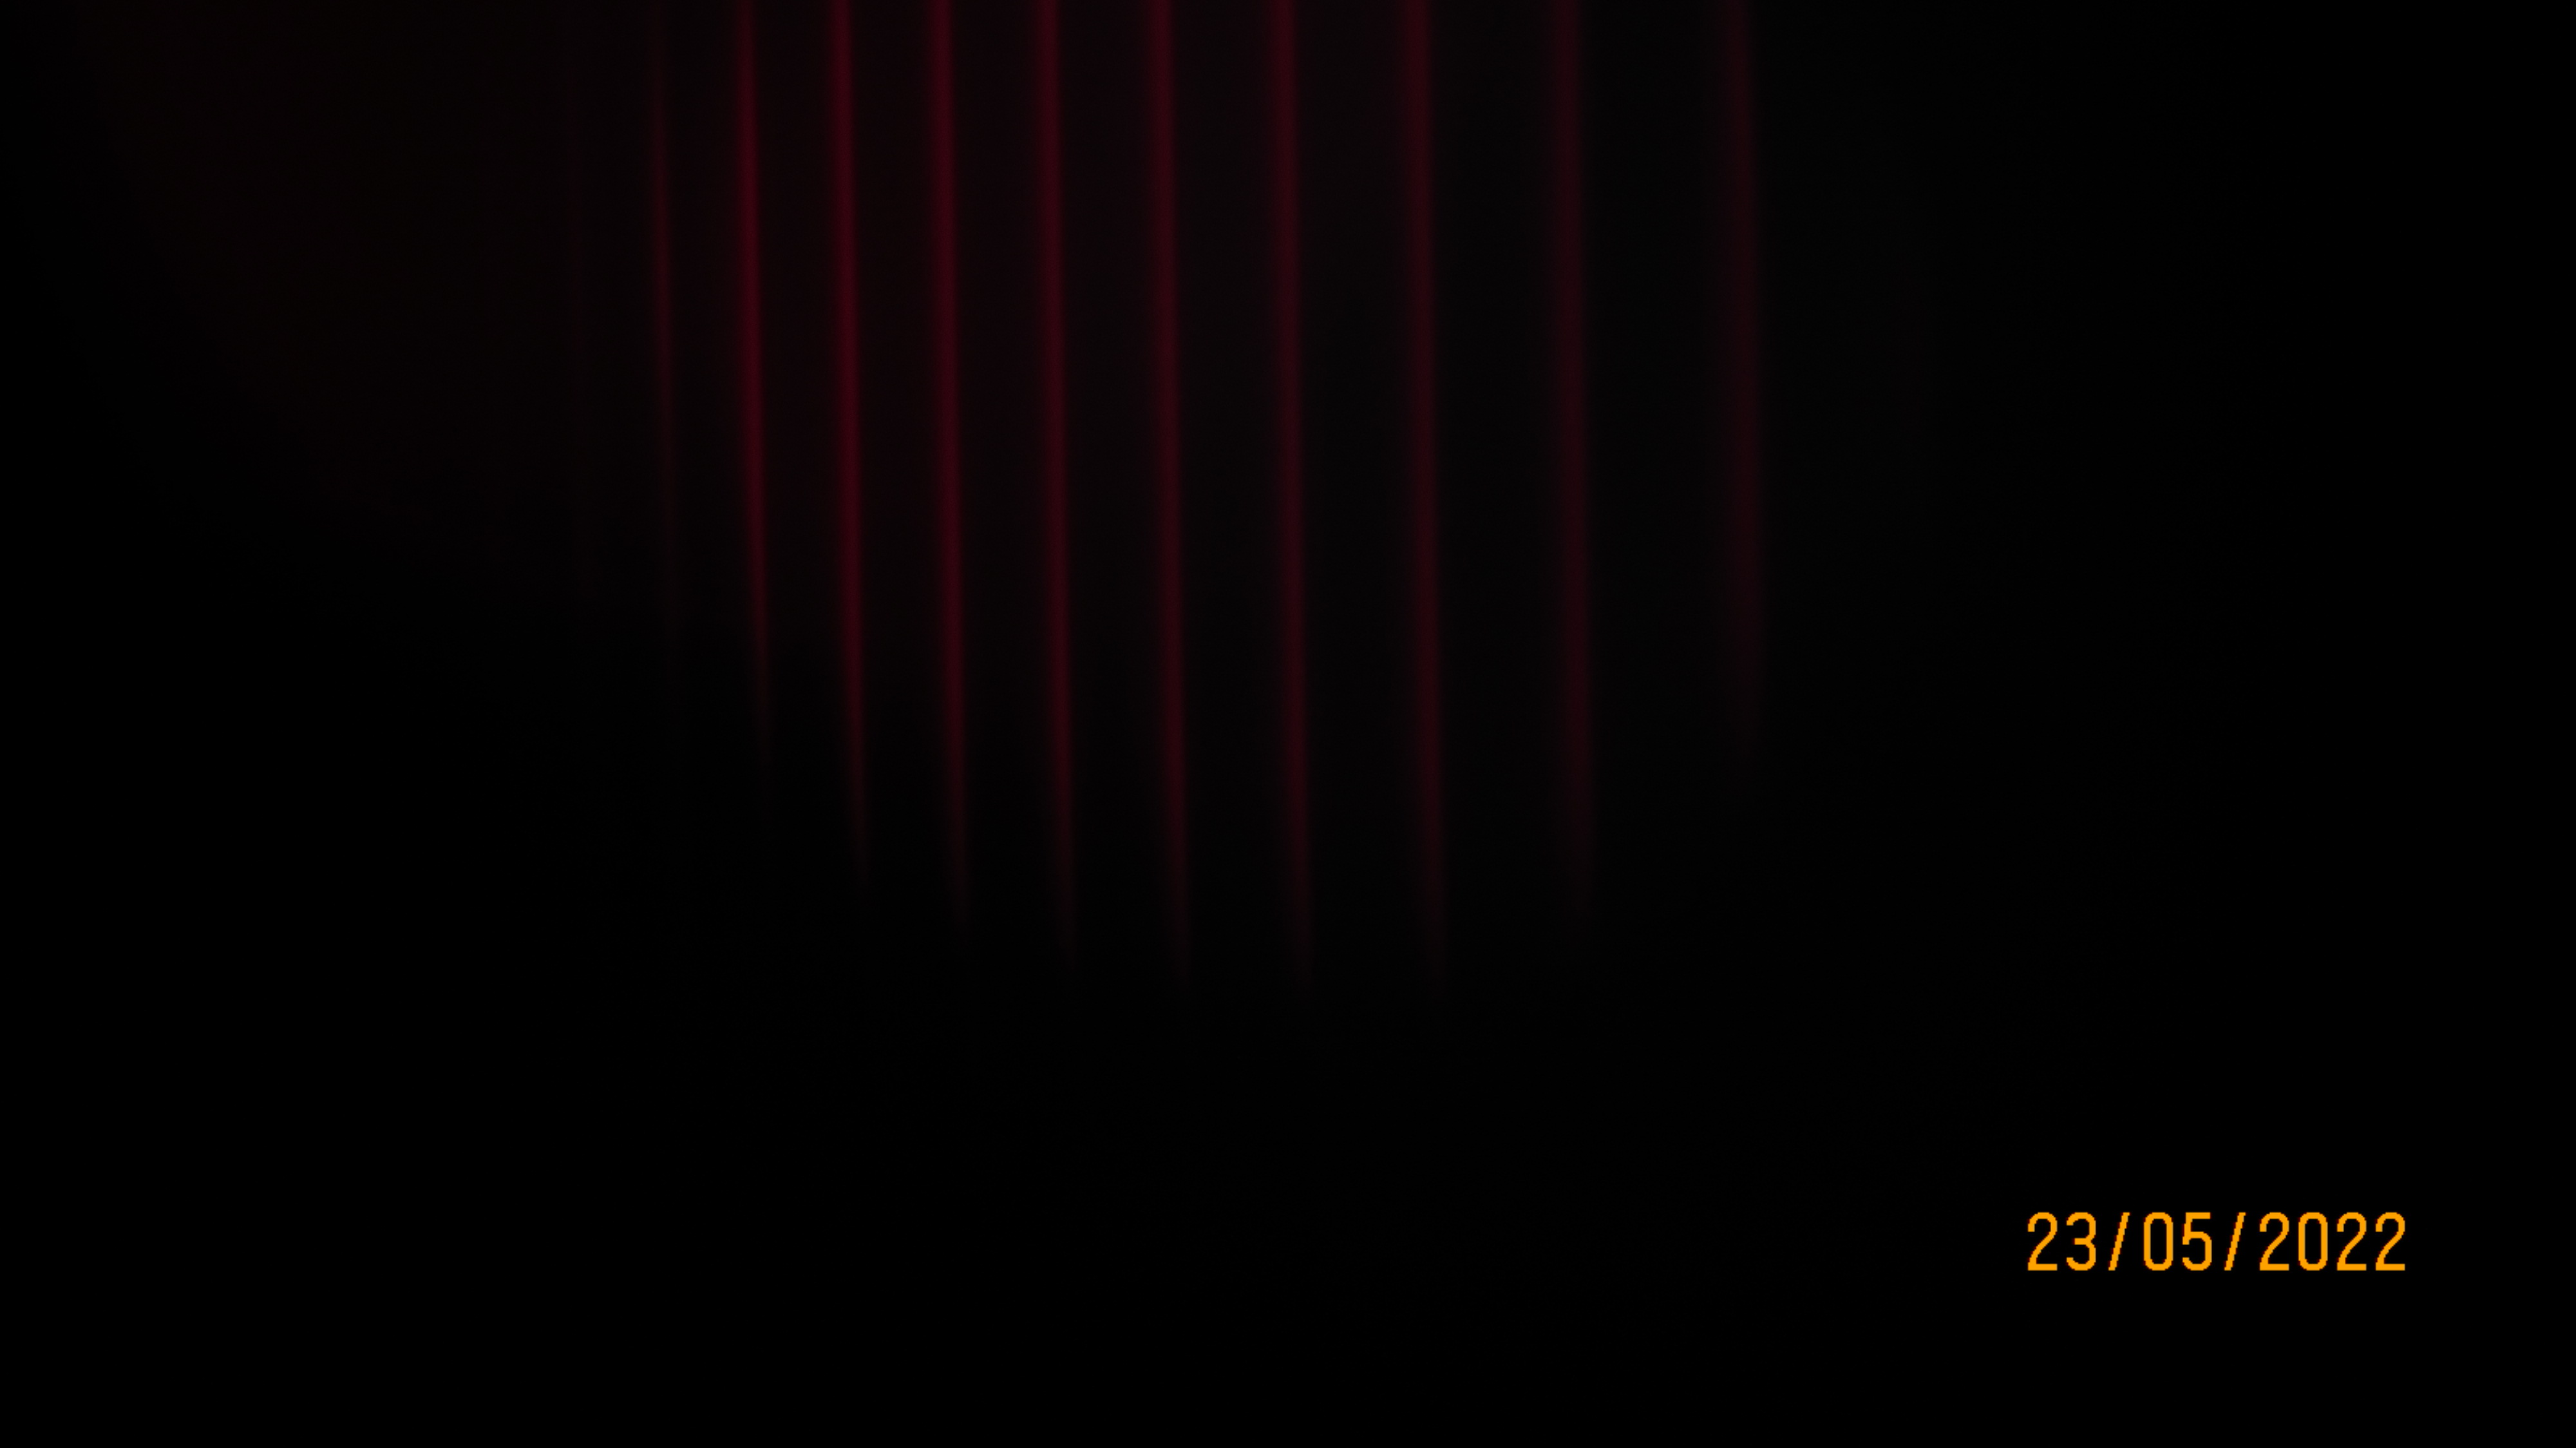
\includegraphics[scale= 0.2]{Messung/Rot[6].JPG}
    \caption{Interferenzmuster der roten Spektrallinie ohne Magnetfeld.}
    \label{fig:rot}
\end{figure}
\noindent

\begin{figure}[H]
    \centering
    
\includegraphics[scale= 0.2]{Messung/Rot_Sigma[7].JPG}
    \caption{Interferenzmuster der roten Spektrallinie beim $\sigma$-Übergang.}
    \label{fig:rot_sigma}
\end{figure}
\noindent
Zur Bestimmung des Lande-Faktors wurden mittels \textit{Affinity Designer} \cite{affinity} die Abstände $\Delta s$ 
in Abbildung \ref{fig:rot} und $\delta s$ in Abbildung \ref{fig:rot_sigma} bestimmt. Die Abstände sind in 
Tabelle \ref{tab:rot} enumeriert.

\begin{table}[H]
    \centering
      \caption{Messwerte für die Linienabstände $\Delta s$ und die Aufspaltung $\delta s$ in Pixeln für die rote Spektrallinie.}
      \label{tab:rot}
      \sisetup{table-format=3.1}
      \begin{tabular}{S[table-format=1.1] S}
        \toprule
        {$\Delta s[\text{px}]$} & {$\delta s[\text{px}]$}\\
        \midrule
        117.9  &  59.2 \\
        128.2  &  56.0 \\
        134.4  &  53.3 \\
        144.6  &  55.1 \\
        149.8  &  63.3 \\
        160.6  &  72.0 \\
        178.7  &  74.7 \\
        202.4  &  84.9 \\
        \bottomrule
      \end{tabular}
\end{table}
\noindent
Die mit \textit{NumPy} \cite{numpy} bestimmten Mittelwerte mit Standardabweichung lauten
\begin{align*}
    \overline{\Delta s}&=\num{152.1\pm 26.0}\text{px}\\
    \overline{\delta s}&=\num{64.81\pm 64.8}\text{px} .
\end{align*}
Einsetzen in Gleichung \ref{eqn:gebiet} ergibt für Dispersionsgebiet
\begin{equation*}
  \delta\lambda=\SI{10.4\pm 2.5}{\pico\metre} .
\end{equation*}
Der Landefaktor $g$ berechnet sich nach Gleichung \ref{eqn:aufspaltung} zu 
\begin{equation*}
  g=\num{0.93\pm0.22} .
\end{equation*}

\subsection{Auswertung der blauen Spektrallinie}
\label{sec:blau}
Für die Untersuchung des anormalen Zeeman-Effekts werden zwei verschiedene Magnetfeldstärken verwendet, um 
die $\pi$- von den $\sigma$-Übergängen unterscheiden zu können. Die Bestimmung von $\Delta s$ wird für beide 
Übergänge an Abbildung \ref{fig:blau} vorgenommen. 

\begin{figure}[H]
    \centering
    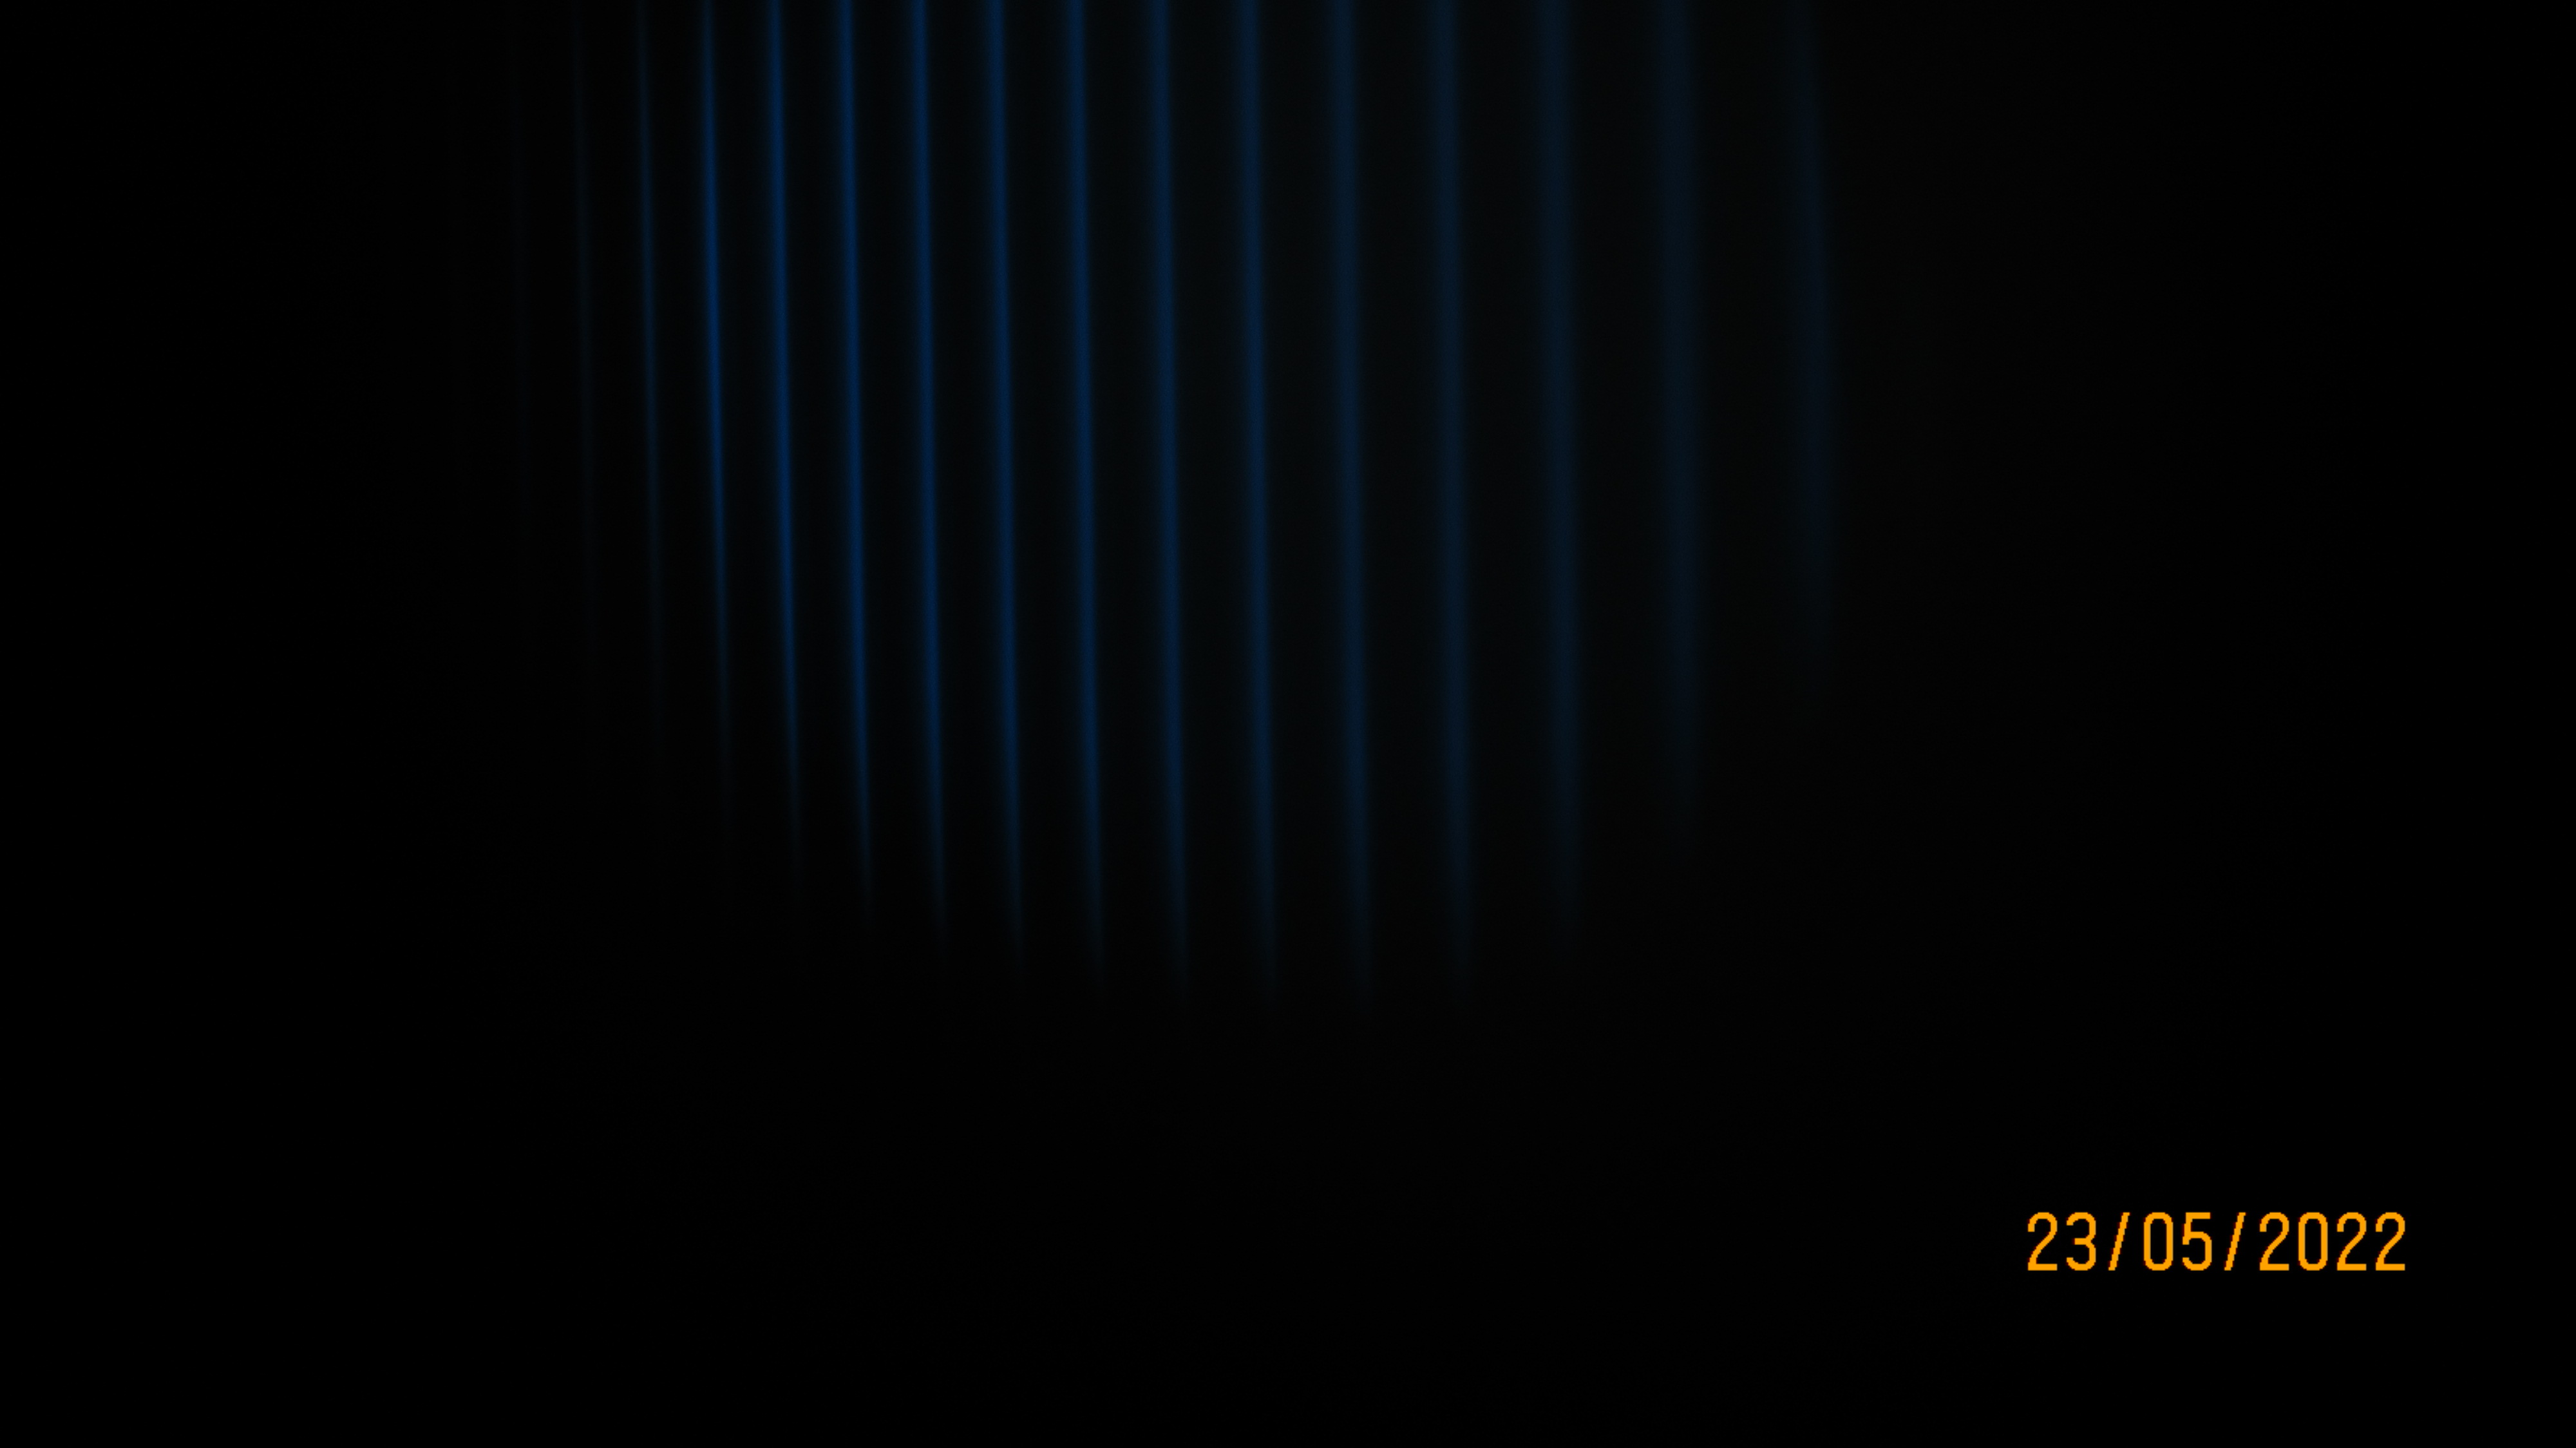
\includegraphics[scale= 0.2]{Messung/Blau[3].JPG}
    \caption{Interferenzmuster der blauen Spektrallinie ohne Magnetfeld.}
    \label{fig:blau}
\end{figure}
\noindent

\subsubsection[]{$\sigma$-Übergang}
\label{sec:sigma}

In Abbildung ist Interferenzmuster der blauen Spektrallinie für eine Stromstärke von $I=\SI{4.5}{\ampere}$
dargestellt. Dieser Stromstärke entspricht nach der Regression \ref{eqn:B} eine Feldstärke von 
$B=\SI{426.7}{\milli\tesla}$. 
\begin{figure}[H]
    \centering
    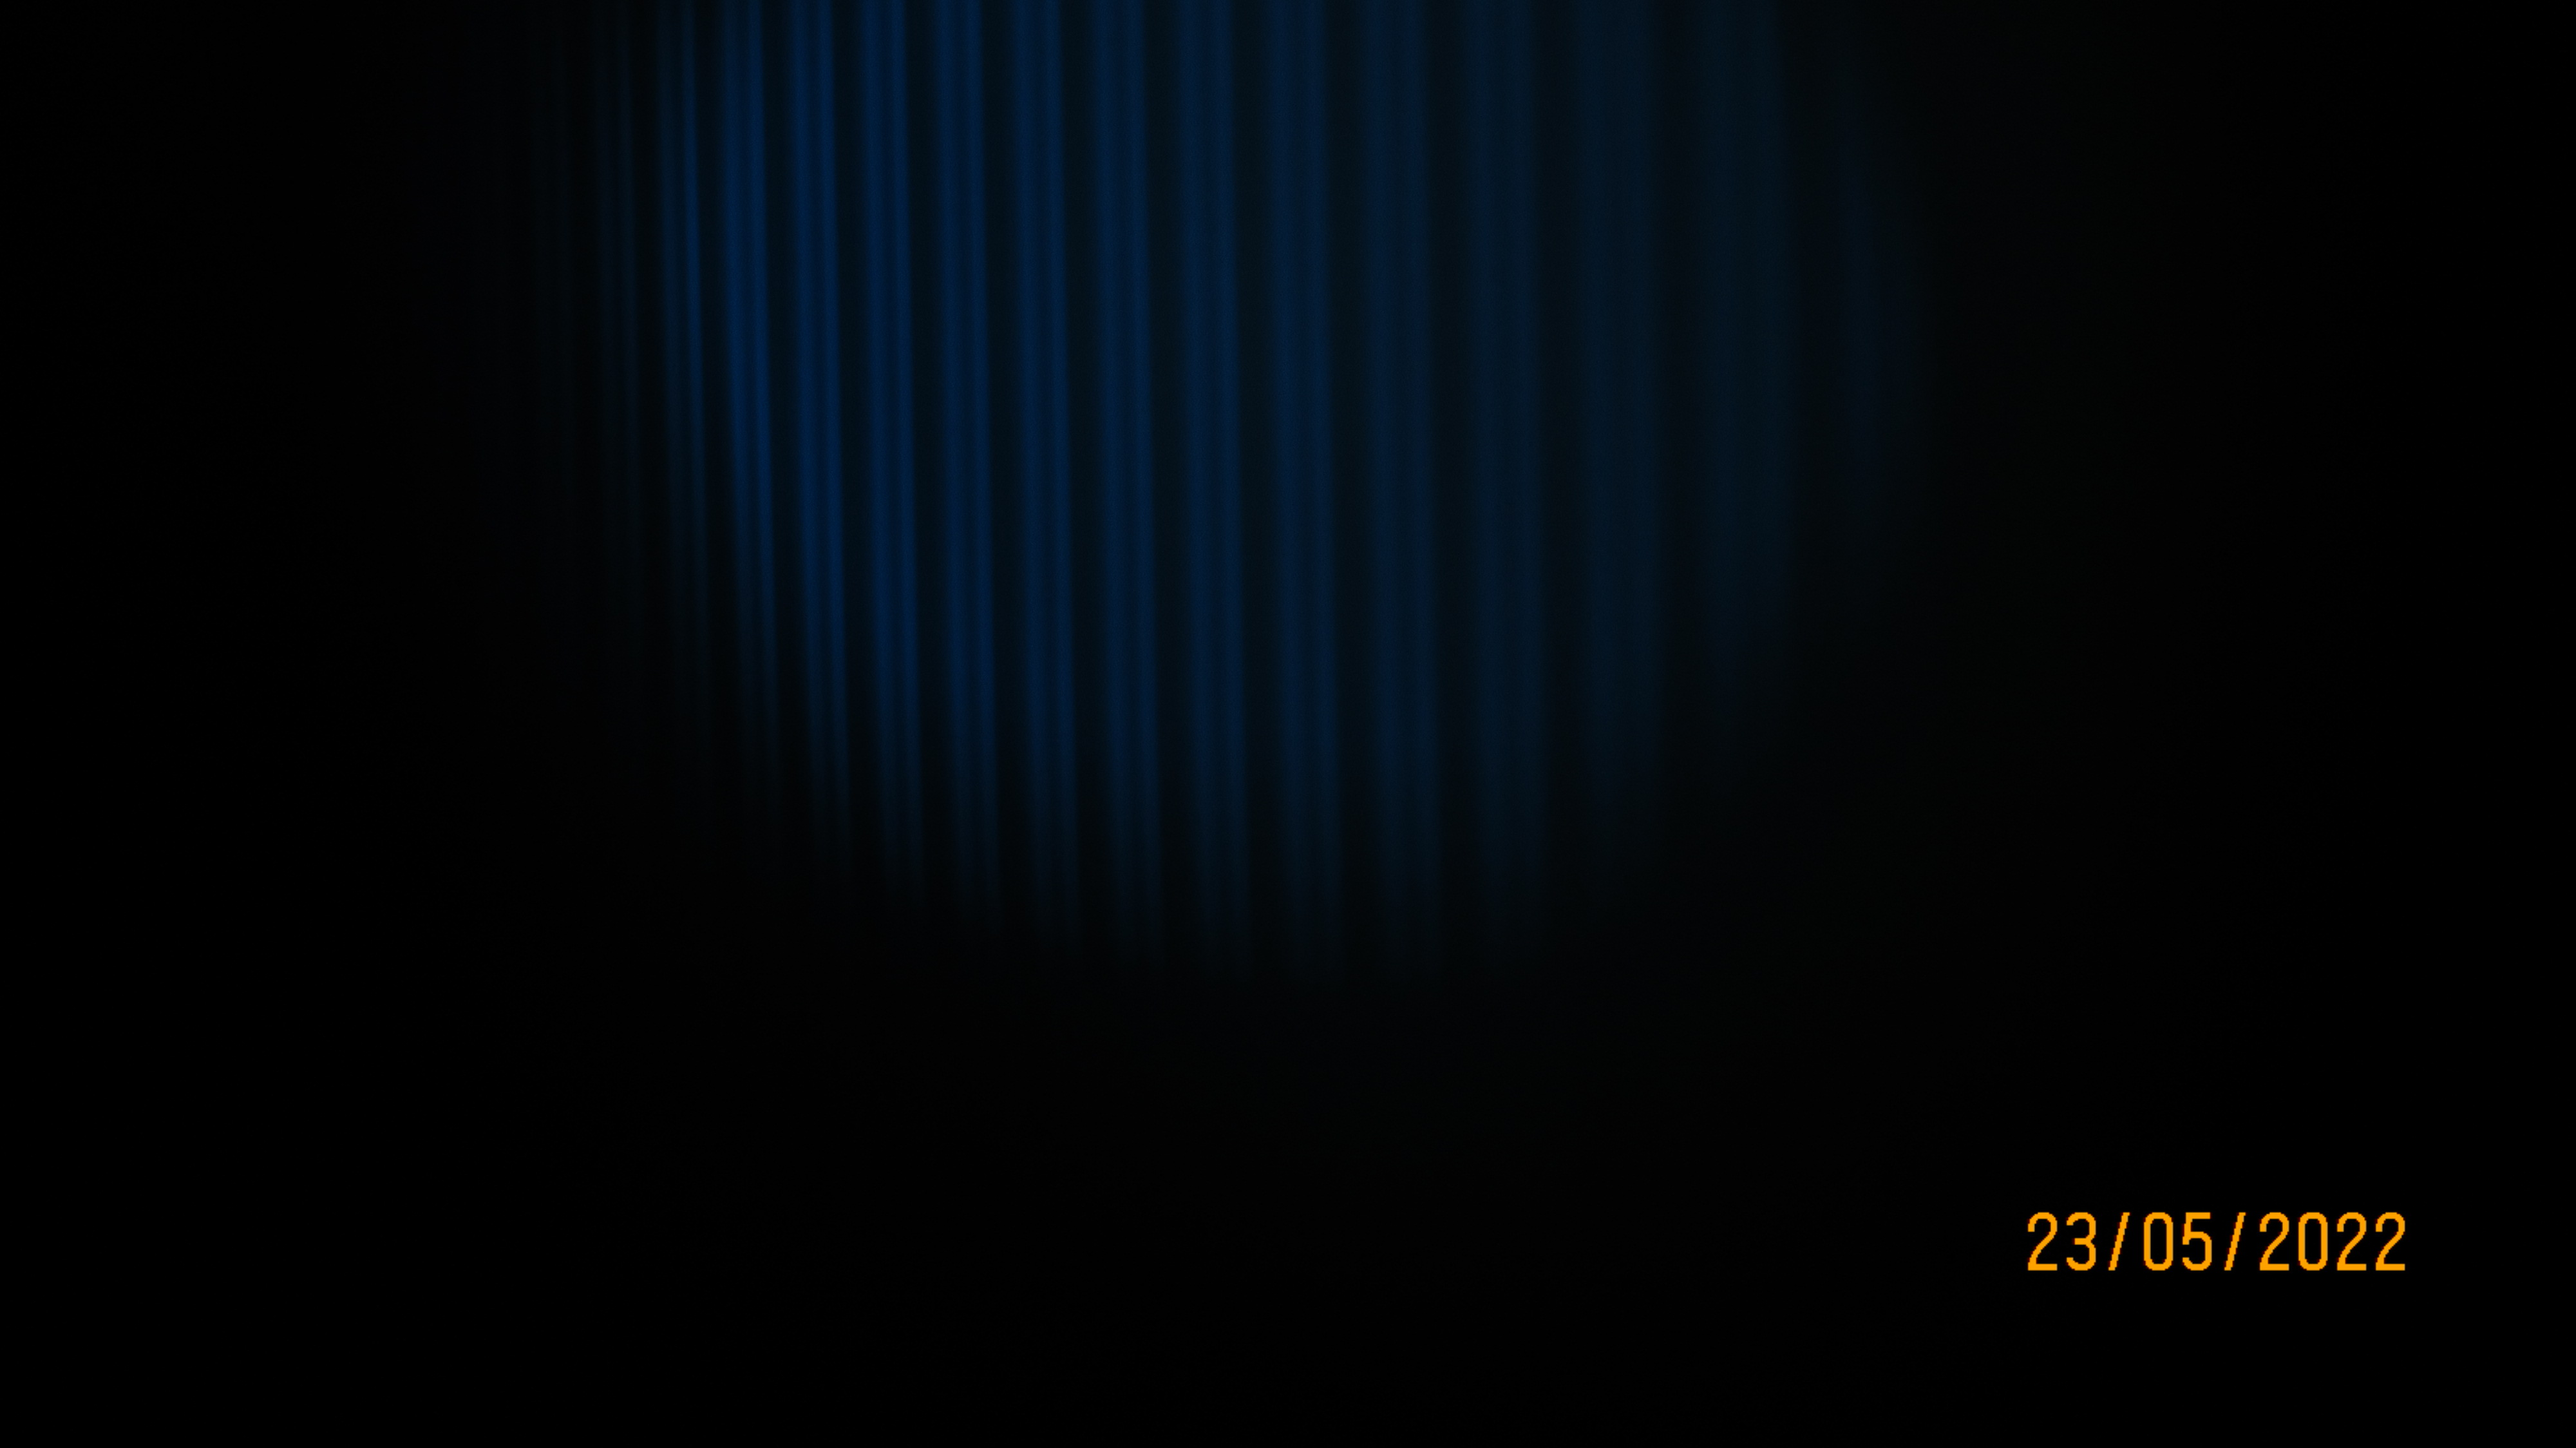
\includegraphics[scale= 0.2]{Messung/Blau_Sigma[4].JPG}
    \caption{Interferenzmuster der blauen Spektrallinie beim $\sigma$-Übergang.}
    \label{fig:blau_sigma}
\end{figure}
\noindent
Die mit \textit{Affinity Designer} \cite{affinity} bestimmten Abstände $\Delta s$ und $\delta s$ sind in Tabelle \ref{tab:blau_sigma}
angeführt.

\begin{table}[H]
    \centering
      \caption{Messwerte für die Linienabstände $\Delta s$ und die Aufspaltung $\delta s$ in Pixeln für den $\sigma$-Übergang der blaue Spektrallinie.}
      \label{tab:blau_sigma}
      \sisetup{table-format=3.1}
      \begin{tabular}{S[table-format=1.1] S}
        \toprule
        {$\Delta s[\text{px}]$} & {$\delta s[\text{px}]$}\\
        \midrule
        84.4  &  30.0 \\
        92.0  &  33.5 \\
        96.8  &  37.0 \\
        99.0  &  38.2 \\
        104.4 &  40.5 \\
        108.0 &  41.8 \\
        114.0 &  44.5 \\
        118.0 &  41.5 \\
        131.0 &  44.4 \\
        140.7 &  47.9 \\
        147.1 &  53.3 \\
        166.0 &  53.2 \\
        190.6 &  55.1 \\
        \bottomrule
      \end{tabular}
\end{table}
\noindent
Doe Mittelwerte werden mit \textit{NumPy} \cite{numpy} als 
\begin{align*}
    \overline{\Delta s}&=\num{122.5\pm 30.1}\text{px}\\
    \overline{\delta s}&=\num{43.2\pm 7.4}\text{px}
\end{align*}
ermittelt. Daraus ergibt sich mit Gleichung \ref{eqn:gebiet} zu 
\begin{equation*}
  \delta\lambda=\SI{4.75\pm 1.42}{\pico\metre},
\end{equation*}
sodass sich der Landefaktor mit Gleichung \ref{eqn:aufspaltung} zu
\begin{equation*}
  g=\num{1.03\pm0.31}
\end{equation*}
bestimmen lässt.

\subsubsection[]{$\pi$-Übergang}
\label{sec:pi}
Das Interferenzmuster \ref{fig:blau_pi} wurde bei einer Stromstärke von $I=\SI{7.5}{\ampere}$ aufgenommenen. 
Der Elektromagnet hat demnach ein Magnetfeld von $B=\SI{577.5}{\milli\tesla}$ erzeugt. 
\begin{figure}[H]
    \centering
    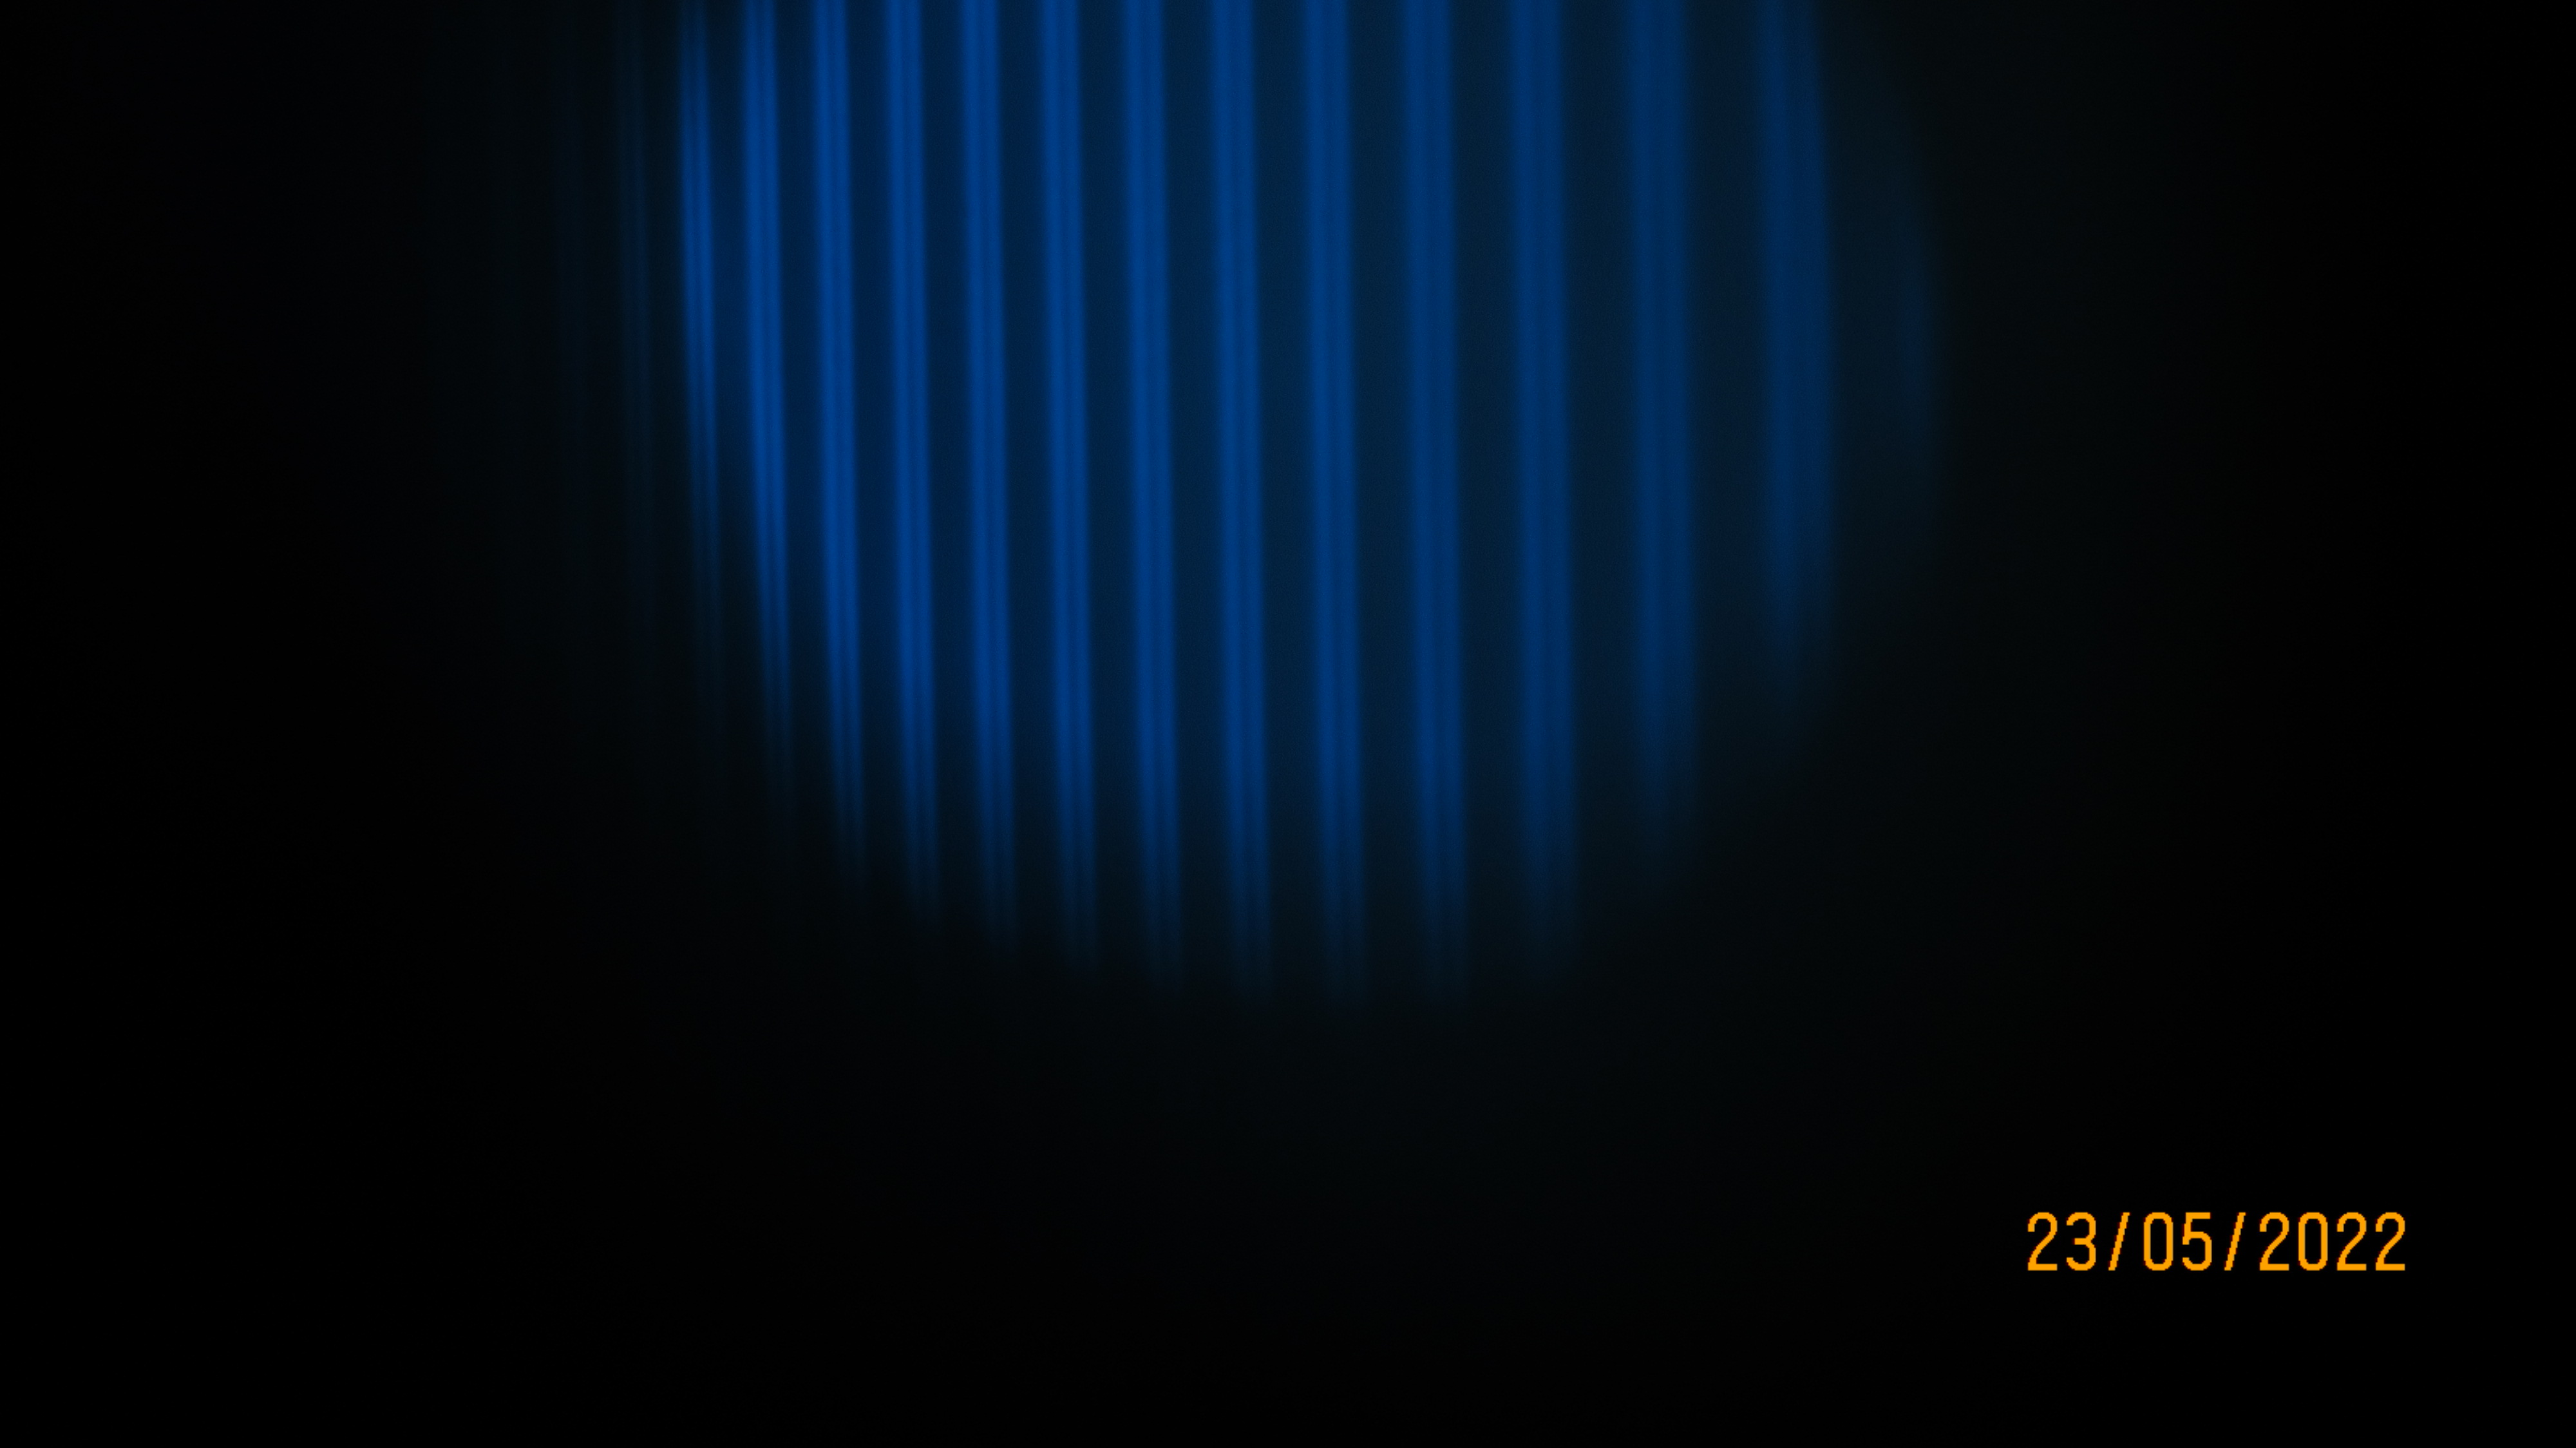
\includegraphics[scale= 0.2]{Messung/Blau_Pi[5].JPG}
    \caption{Interferenzmuster der blauen Spektrallinie beim $\pi$-Übergang.}
    \label{fig:blau_pi}
\end{figure}
\noindent
Die in Tabelle \ref{tab:blau_pi} gelisteten Werte von $\Delta s$ und $\delta s$ wurden erneut mit \textit{Affinity Designer} \cite{affinity}
bestimmt.

\begin{table}[H]
    \centering
      \caption{Messwerte für die Linienabstände $\Delta s$ und die Aufspaltung $\delta s$ in Pixeln für den $\pi$-Übergang der blaue Spektrallinie.}
      \label{tab:blau_pi}
      \sisetup{table-format=3.1}
      \begin{tabular}{S[table-format=1.1] S}
        \toprule
        {$\Delta s[\text{px}]$} & {$\delta s[\text{px}]$}\\
        \midrule
        84.4  &  30.0 \\
        92.0  &  33.5 \\
        96.8  &  37.0 \\
        99.0  &  38.2 \\
        104.4 &  40.5 \\
        108.0 &  41.8 \\
        114.0 &  44.5 \\
        118.0 &  41.5 \\
        131.0 &  44.4 \\
        140.7 &  47.9 \\
        147.1 &  53.3 \\
        166.0 &  53.2 \\
        190.6 &  55.1 \\
        \bottomrule
      \end{tabular}
\end{table}
\noindent
Die Mittelwerte der Messwerte sind 
\begin{align*}
    \overline{\Delta s}&=\num{122.5\pm 30.1}\text{px}\\
    \overline{\delta s}&=\num{33.6 \pm 10.5}\text{px},
\end{align*}
woraus sich ein Dispersionsgebiet von 
\begin{equation*}
  \delta\lambda=\SI{3.70\pm 1.47}{\pico\metre}
\end{equation*}
ergibt. Dies führt schlussendlich nach Gleichung \ref{eqn:aufspaltung} zu einem Landefaktor von 
\begin{equation*}
  g=\num{0.60\pm 0.24} .
\end{equation*}